\begin{tikzpicture}
    % Réduit l'interligne
    \linespread{0.7}
    
    % Inclus l'image
    \node[anchor=south west,inner sep=0] (image) at (0,0) {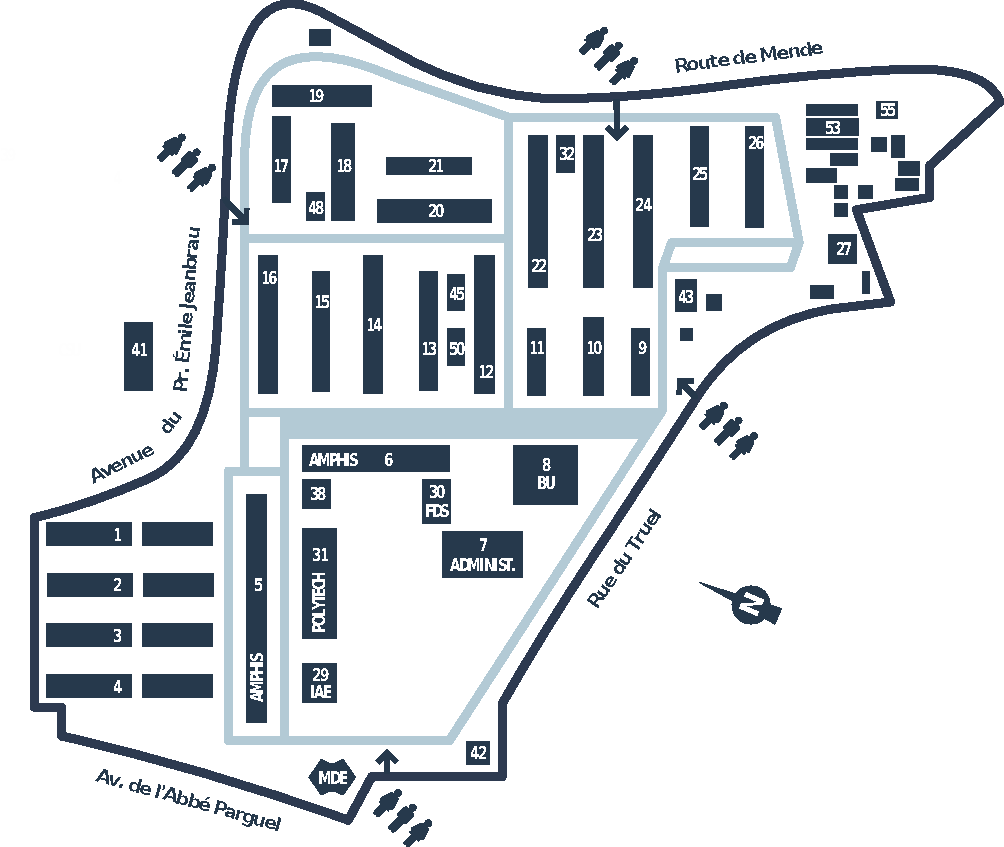
\includegraphics[trim={9.4cm 9cm 0cm 0cm},clip,scale=1.3]{images/plan.pdf}};
    
    % Définitition des styles
    \tikzstyle{wasp}        = [black]
    \tikzstyle{waspRelais}  = [wasp,fill=blue]
    \tikzstyle{waspCapt}    = [wasp,fill=yellow]
    \tikzstyle{waspBoth}    = [wasp,fill=OliveGreen]
    \tikzstyle{conn}        = [OliveGreen,ultra thick,dotted]
    \tikzstyle{bat}         = [red,ultra thick]
    \tikzstyle{legend}      = [anchor=west,text=darkgray]
    \tikzstyle{onMap}       = [anchor=center,text=red,text width=2.5cm,align=center]

    % Zone de dessin
    \begin{scope}[x={(image.south east)},y={(image.north west)}]
        % Grille
        %\draw[help lines,xstep=.05,ystep=.1] (0,0) grid (1,1);
        
        % Repère
        %\foreach \x in {0,1,...,9} { \node [anchor=north] at (\x/10,0) {0.\x}; }
        %\foreach \y in {0,1,...,9} { \node [anchor=east] at (0,\y/10) {0.\y}; }
        
        % Animalerie
        \draw[bat,rounded corners] (0.55,0.51) rectangle (0.688,0.68);
        \node[onMap] at (0.63,0.72) {Animalerie};
        
        % Bâtiment de recherche
        \draw[bat,rounded corners] (0.166,0.08) rectangle (0.225,0.58);
        \node[onMap] at (0.17,0.042) {Bâtiment de recherche};
        
        % Connections
        \draw[conn] (0.445,0.500)  --  (0.322,0.5);     % R3 -- R2
        \draw[conn] (0.322,0.500)  --  (0.198,0.5);     % R2 -- R1
        \draw[conn] (0.578,0.595)  --  (0.445,0.5);     % R3 -- M
        \draw[conn] (0.620,0.650)  --  (0.578,0.595);   % C1 -- M
        \draw[conn] (0.620,0.542)  --  (0.578,0.595);   % C3 -- M
        \draw[conn] (0.660,0.595)  --  (0.578,0.595);   % C2 -- M

        % Waspmotes
        \draw[waspRelais] (0.445,0.500)  circle  (0.14cm);  % R3
        \draw[waspRelais] (0.322,0.500)  circle  (0.14cm);  % R2
        \draw[waspRelais] (0.198,0.500)  circle  (0.14cm);  % R1
        \draw[waspCapt]   (0.620,0.650)  circle  (0.14cm);  % C1
        \draw[waspCapt]   (0.620,0.542)  circle  (0.14cm);  % C3
        \draw[waspCapt]   (0.660,0.595)  circle  (0.14cm);  % C2
        \draw[waspBoth]   (0.578,0.595)  circle  (0.14cm);  % M

        % Légende
        \footnotesize
        \draw[darkgray] (0.775,-0.02) rectangle (1.15,0.32);
        \node[anchor=center,text=darkgray] at   (0.91,0.28) {\bfseries\underline{\textit{Légende}}};
        \draw[waspRelais]    (0.80,0.22) circle (0.14cm);
        \node[legend] at     (0.82,0.22) {Waspmote relais};
        \draw[waspCapt]      (0.80,0.17) circle (0.14cm);
        \node[legend] at     (0.82,0.17) {Waspmote capteur};
        \draw[waspBoth]      (0.80,0.12) circle (0.14cm);
        \node[legend] at     (0.82,0.12) {Waspmote mère};
        \draw[conn]          (0.785,0.07) -- (0.815,0.07);
        \node[legend] at     (0.82,0.07) {Connexion};
        \draw[bat,thick]     (0.785,0.005) rectangle (0.815,0.035);
        \node[legend] at     (0.82,0.020) {Bâtiment clef};
    \end{scope}
\end{tikzpicture}